
\documentclass[book.tex]{subfiles}
\begin{document}
\label{chapter_team}
In 1990 a small company based in Shreveport, Louisiana was doing well in the shareware market. As a video game subscription service, Softdisk produced and mailed new games every month to its members. Business was good but some of its employees had other ambitions. They thought they had the skills to make it big and they wanted to prove it.\\
\par
They had created a new way to program side scrolling. They called the technology "adaptive tile refresh" and it enabled hardware scrolling on a PC capable of rivaling a NES. In early 1990 they worked non-stop over a weekend to reimplement Super Mario 3 on a PC and demonstrate their skills to Nintendo. The team was successful in building a clone of Mario, but unfortunately "Ideas from the Deep" as they called themselves failed to convince Nintendo to give them a contract.\\
\par As impressed as they were, the Japanese firm wanted the Mario series to remain exclusive to Nintendo consoles.\\
\par
\begin{fancyquotes}
We sent this demo to Nintendo of America, they in turn sent it to Kyoto to the mothership office, and the execs there saw the demo and were really impressed. However, they didn't want their intellectual property on anything but their own hardware, so they told us Good Job and You Can't Do This\protect\footnotemark.
 \bigskip \\
\textbf{John Romero - Programmer}
 \end{fancyquotes}
\footnotetext{Super Mario Bros. 3 Demo (1990) by John Romero: https://vimeo.com/148909578}
 \begin{figure}[H]
   \fullimage{mario_ifd.png}
\caption{Mario 3 on PC. Notice the "IFD" for "Ideas From the Deep".}
\end{figure}

\par
This episode was enough to convince them they had not only the talent to feed their ambitions, but also the teamwork and work ethic to potentially go all the way. In February 1991 four Softdisk employees took the leap of faith and founded their own company: "id Software"\footnote{For ample details, read "Masters of Doom" by David Kushner.}.\\ 
\par
 
 \begin{figure}[H]
\centering  
\begin{tabularx}{\textwidth}{ X  X  X  }
  \toprule
  \textbf{Name} &  \textbf{Age} & \textbf{Occupation} \\
  \toprule 
   John Carmack & 21 &  Programming\\
   John Romero & 25 &  Programming\\
   Adrian Carmack & 22 &  Artist\\
   Tom Hall & 28 &  Creative Director\\
     \toprule
\end{tabularx}
\caption{id Software founding members.}\label{fig:Id Software team}
\end{figure}
\pagebreak
They immediately used the technology developed for "Mario 3 PC" to release their own titles and build their own intellectual property. Wasting no time, the team shipped no less than three titles annually.
\begin{itemize}
    \item Commander Keen Episode 1, 2, and 3: Invasion of the Vorticons (December 14th, 1990)
    \item Commander Keen Episode 4, 5, and 6: Good Bye Galaxy (December 15th, 1991)
    \item Commander Keen standalone game: Aliens Ate My Baby Sitter (December 1991)
\end{itemize}
The games, published by FormGen, were instant successes and sold very well. They also kept on writing games for Softdisk to publish, most of which featured adaptive tile refresh:
\begin{itemize}
  \item Commander Keen in Keen Dreams (1991)
  \item Dangerous Dave in the Haunted Mansion (1991)
  \item Rescue Rover (1991)
  \item Rescue Rover 2 (1991)
  \item Shadow Knights (1991)
  \item Hovertank 3D (April, 1991).
  \item Catacomb 3D: A New Dimension (November, 1991)
\end{itemize}
During Spring of 1991 the next generation of id Software technology started to surface\footnote{You can see screenshots in the Annex section on page \pageref{hovertank3d_screenshot} and \pageref{catacomb3d_screenshot}.}. Hovertank 3D placed the player inside a tank. There was no texture mapping yet and the pace was quite slow. Catacomb 3D marked the introduction of textures and took immersion one step further by placing the player in control of a magician in first person view. \\
\par

In November 1991, the team was free from any obligations to SoftDisk. Their next game was going to feature the 3D technology they were building and would be called Wolfenstein 3D. Given the magnitude and ambition of the title, four more people were added to the team for a total of eight.\\
%\note{TODO Ask team members if they know how old were Jay, Bobby, Robert and Jason}
 \begin{figure}[H]
\centering  
\begin{tabularx}{\textwidth}{ X  X  X  }
  \toprule
  \textbf{Name} &  \textbf{Age} & \textbf{Occupation} \\
  \toprule 
   Jay Wilbur & 30 &  Business\\
   Kevin Cloud\protect\footnotemark & 27 &  Computer Artist\\
   Robert Prince\protect\footnotemark & 37 &  Composer\\
   Jason Blochowiak\protect\footnotemark & ?? &   Programming\\
     \toprule
\end{tabularx}
%\caption{id Software hires/contractors.}
\label{fig:Id Software hires}
\end{figure}
\addtocounter{footnote}{-2}
\footnotetext{Jay and Kevin were recruited on April 1st, 1992 but were still given credit for participating in the game development.}
\stepcounter{footnote}
 \footnotetext{Robert had worked with id Software before on Keen 4-6. He remained a contractor, and was never a full-time employee.}
 \stepcounter{footnote}
 \footnotetext{Jason wrote part of the page manager and is credited for introducing John Carmack to Unix development, which ultimately led to the purchase of a Next ColorStation.}

\begin{fancyquotes}
Jason was part of id at the start, but we parted ways during Wolf development.
 \bigskip \\
\textbf{John Carmack - Programmer}
 \end{fancyquotes}


 
\begin{figure}[H]
\centering
  
      \fullimage{idTeam_team_pants.png}
    

\label{fig:id_team_1993}
\end{figure}
\par
Above is the team as shown in Spear of Destiny, in an Easter Egg created by John Romero. To view this screen, the player had to go in the Change View menu, hold down I and D on the keyboard, and press Escape.

\begin{figure}[H]
\centering
  
      \fullimage{id_team_with_pants.jpg}
    
\caption{They were in fact wearing pants.}
\label{fig:id_team_1993}
\end{figure}

\section{Organization}

In September 1991, following Tom and Jason's high-school memories of the area, the team relocated from Shreveport, LA to Madison, WI. They established their office in a two story brick building at 2622 in The Pines complex on High Ridge Trail. They all lived in walking distance of the office except for John Carmack who, since he did not care, inherited of the second floor of the building.\\
\par
The development of Wolfenstein 3D started in November 1991. As temperatures fell and snow dumped from the sky, the team kept itself increasingly busy and barely left the office. Development lasted seven months and Wolfenstein 3D was released in May 1992.

\begin{figure}[H]
\centering
 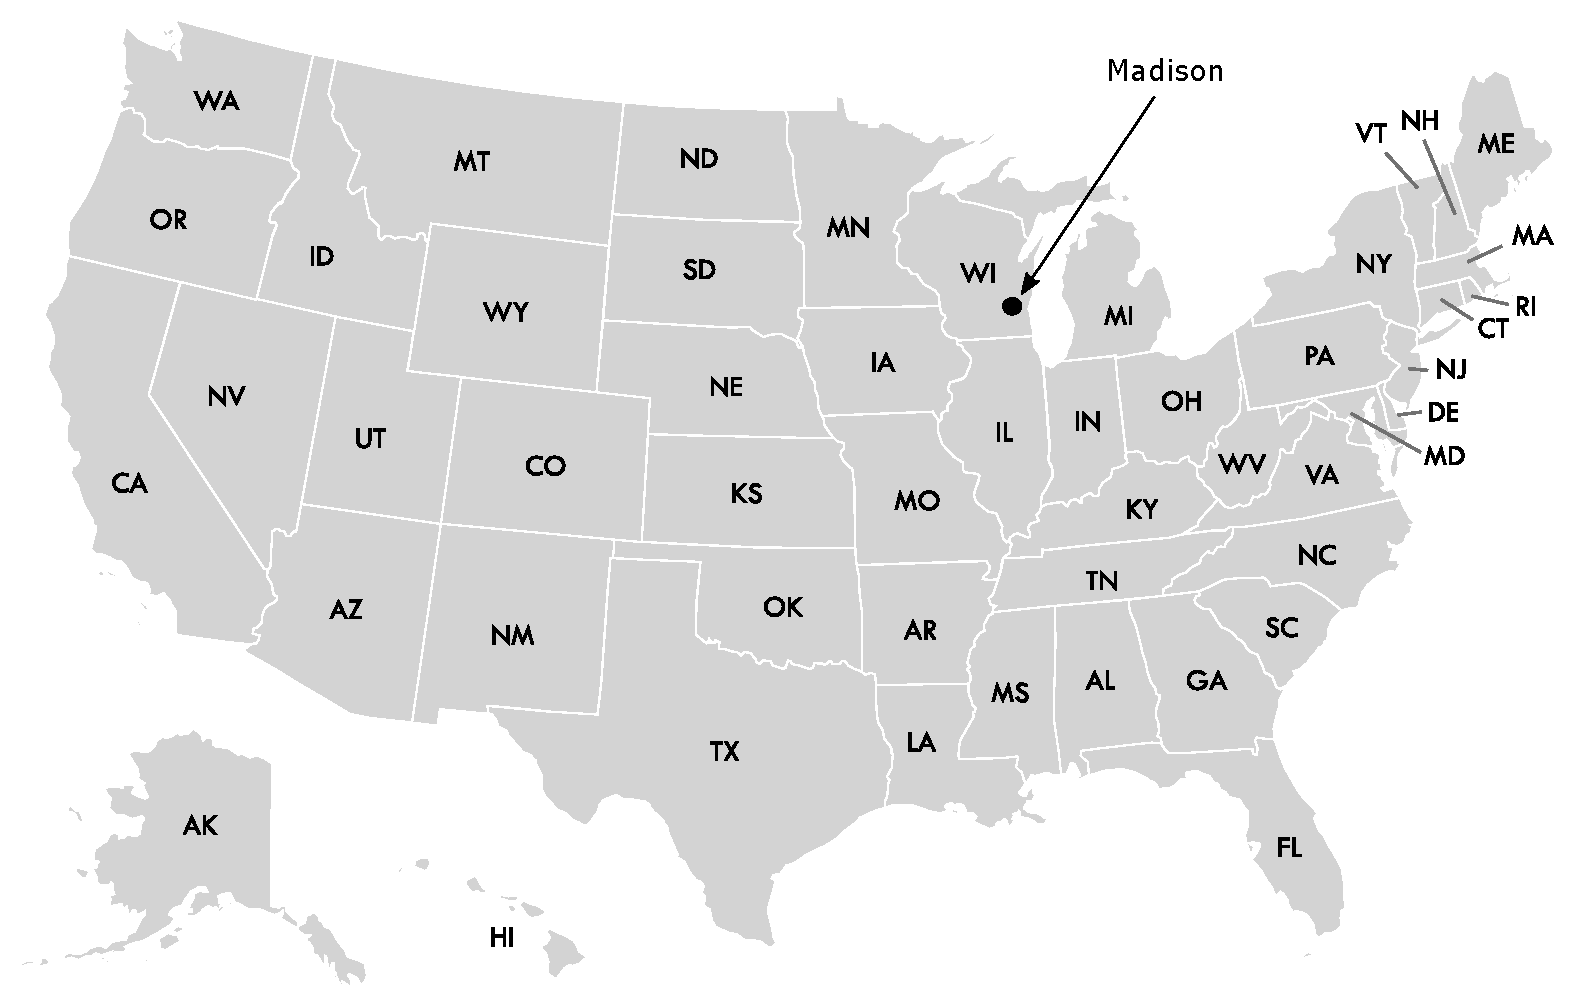
\includegraphics[width=\textwidth]{imgs/drawings/map/usa-id-software.eps}
 \end{figure}


\par

During these seven months, the organization of the team was pretty much standard for a game studio of this era: four guys crammed in one room, dictating a fast pace and strong sense of camaraderie (and a lot of noise disturbance given John Romero and Tom Hall's type of interaction).\\
\par On the map (next page) you can see on the upper floor the SNES where countless games of F-Zero were played and the Dungeons \& Dragons area extensively mentioned in "Masters of Doom". To have a team member (John Carmack) with his apartment directly above the studio was not out of the ordinary\footnote{ "90 Hours A Week And Loving It!" by Andy Hertzfeld.}.\\
\par
\begin{fancyquotes}
We started with floppy data transfer, but we had a Novell network on coax Ethernet by the end. We didn't have a version control system.  Surprisingly, we went all the way to Quake 3 without one, then we started using Visual Source Safe.\\
 \\
\textbf{John Carmack - Programmer}
\end{fancyquotes}







\par
\begin{figure}[H]
  \centering
  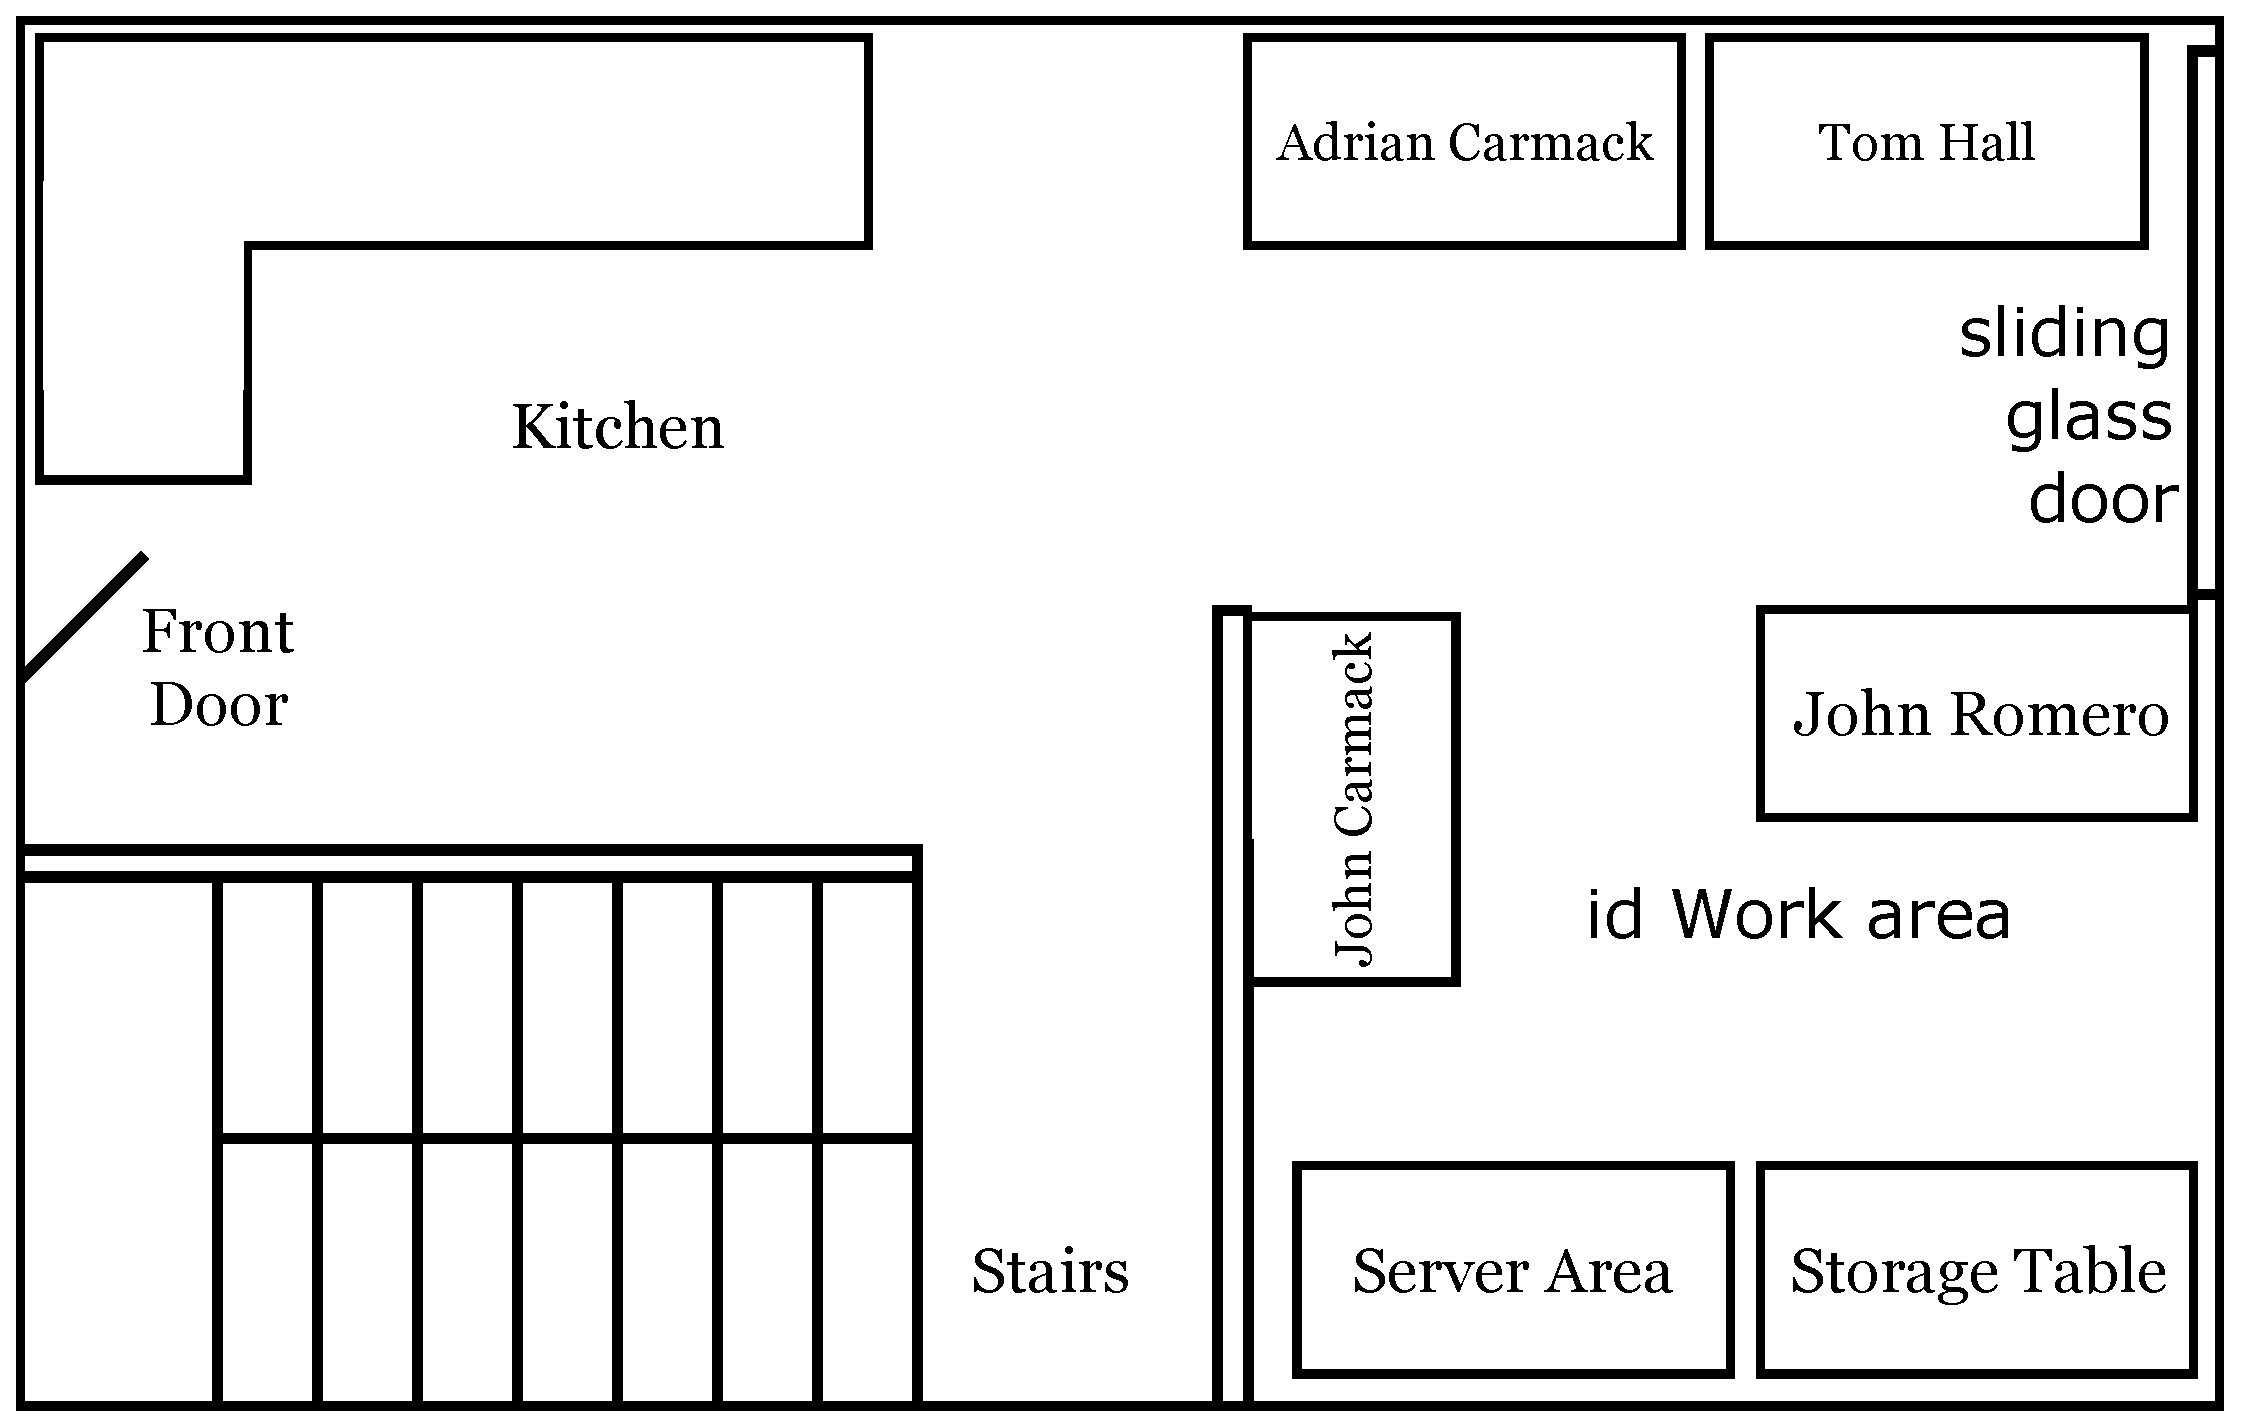
\includegraphics[width=\textwidth]{imgs/drawings/map/id-software-office-madison_bottom_floor.eps}
 %\caption{Office bottom floor.} 
\end{figure}
\par
\begin{figure}[H]
  \centering
  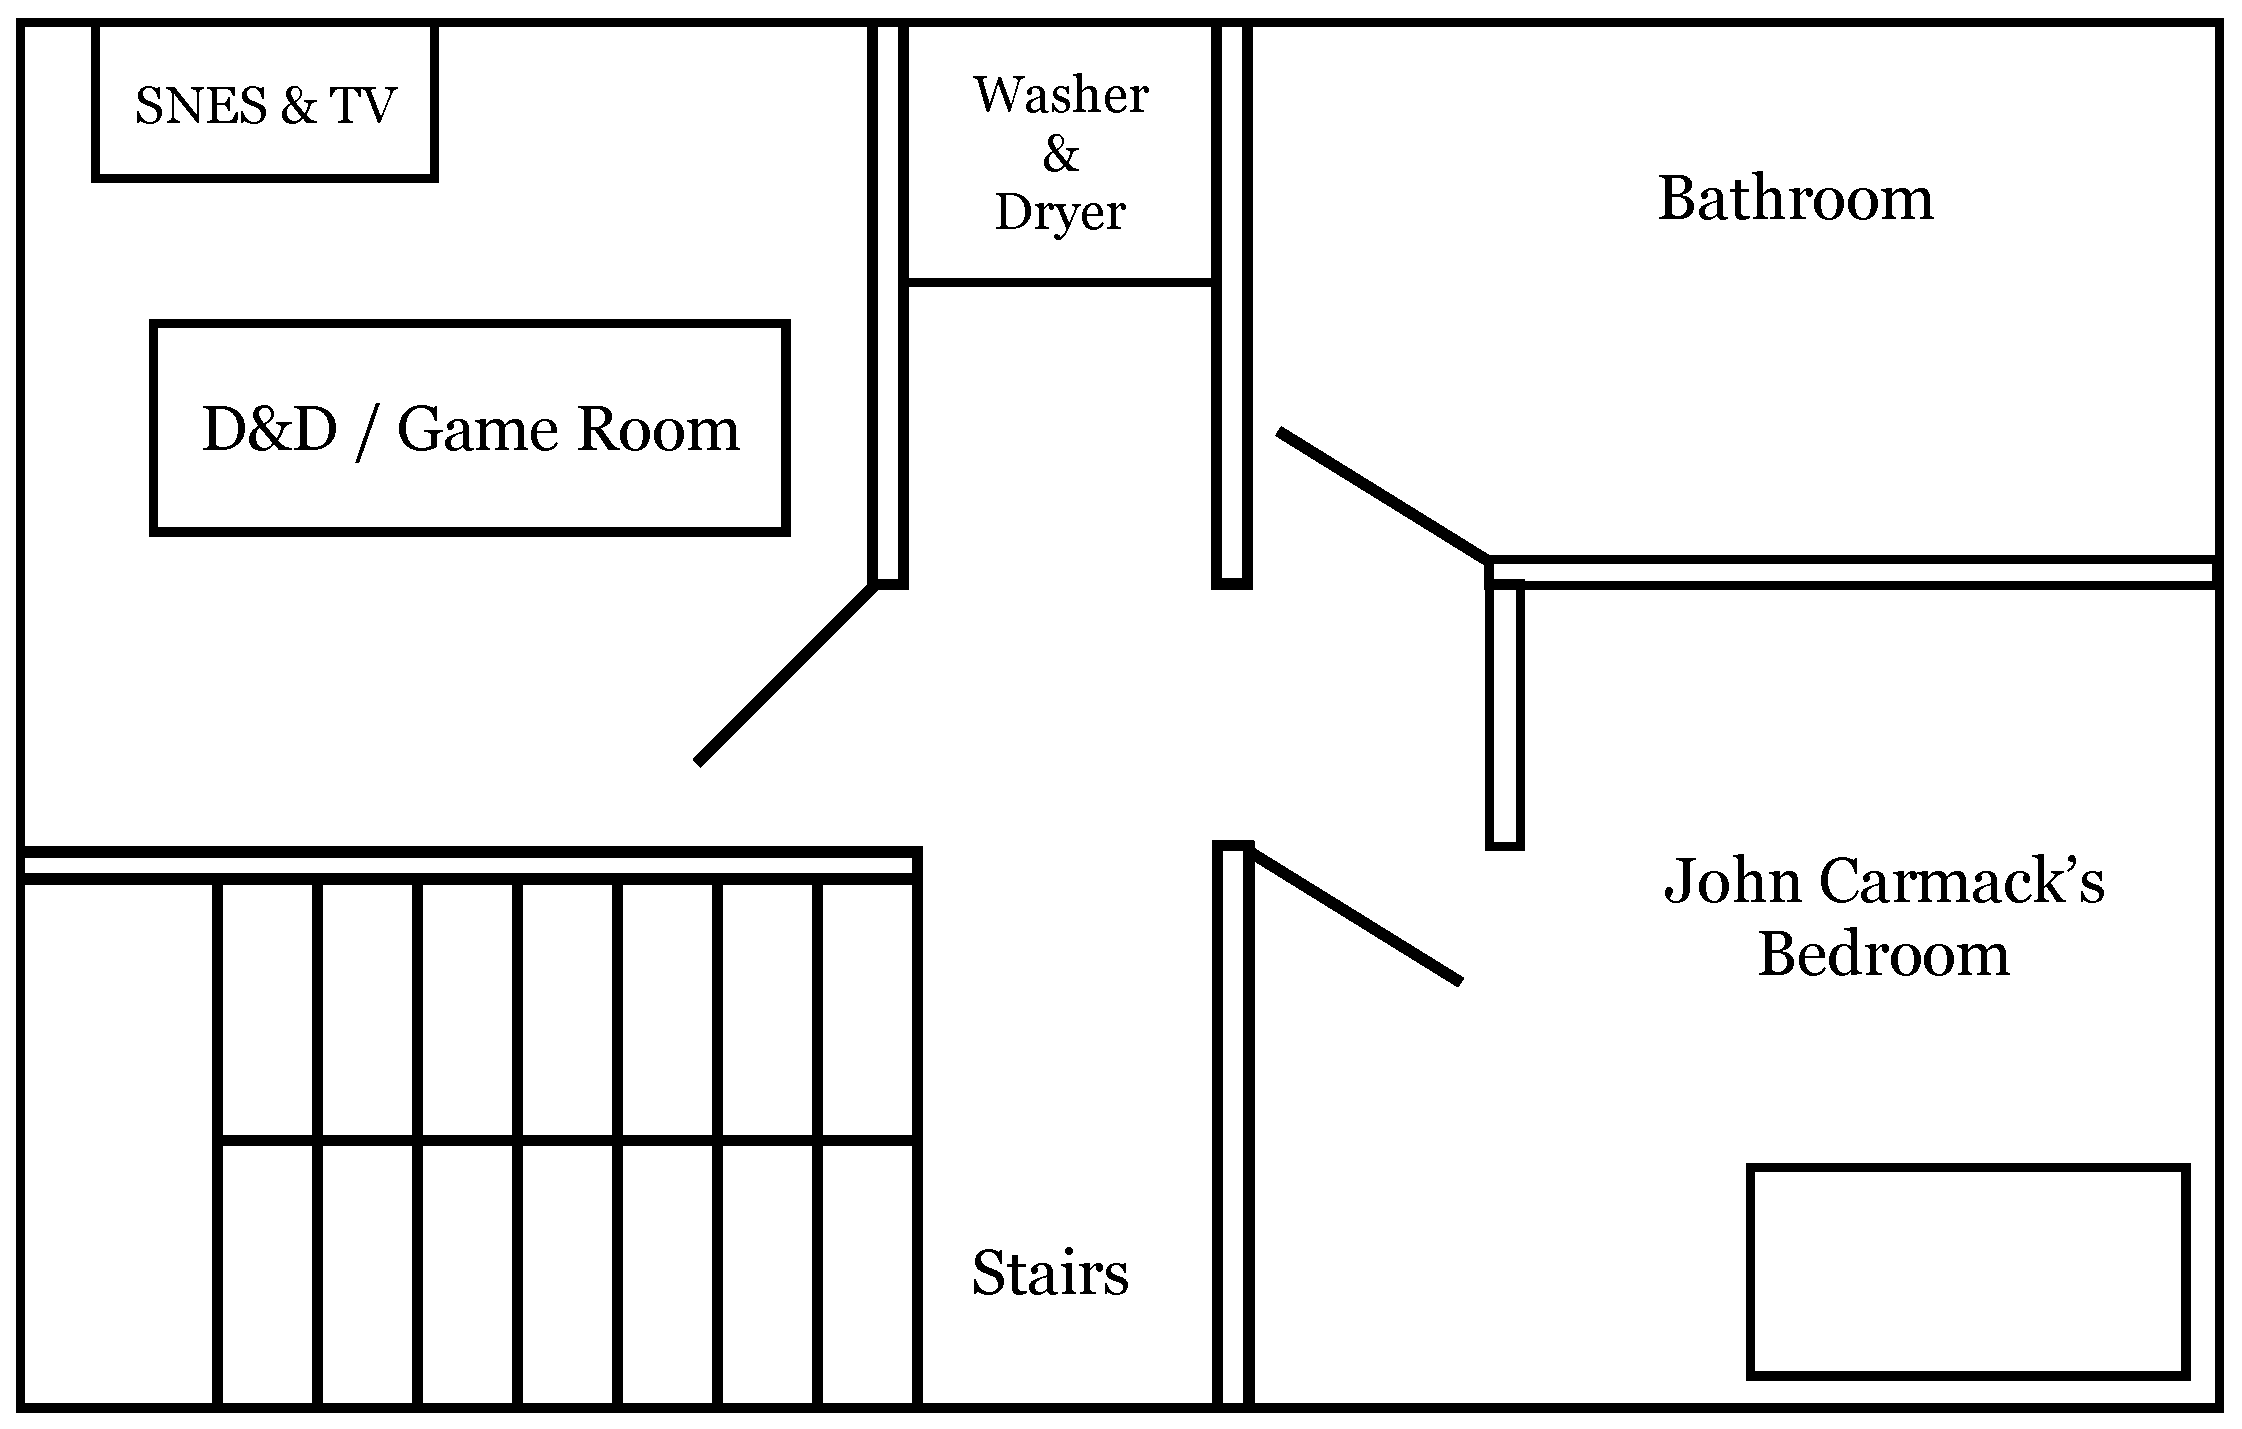
\includegraphics[width=\textwidth]{imgs/drawings/map/id-software-office-madison_top_floor.eps}
 %\caption{Office top floor.} 
\end{figure}

\pagebreak
Everybody was working with the best PC money could buy, a high end 386-DX 33Mhz with 4MiB of RAM.\\

 


























\section{Programming}



Development was done with Borland C++ 3.1 (but the language used was C) which ran in VGA mode 3 offering a screen 80 characters wide and 25 characters tall.\\
\par
John Carmack took care of the runtime code. John Romero programmed many of the tools (TED5 map editor, IGRAB-ED graphic assets packers, MUSE sound packer). Jason Blochowiak wrote important subsystems of the game (Input manager, Page manager, Sound manager, User manager).\\

\begin{figure}[H]
\centering
  \fullimage{development.png}
\caption{Borland C++ 3.1 editor}
\end{figure}
\par
Borland solution was an all-in-one package. The IDE, \cw{BC.EXE}, despite some instabilities allowed crude multi-windows code editing with pleasant syntax highlights. Compiled and Linker were also part of the package under \cw{} and \cw{TLINK.EXE}\footnote{Source: Borland C++ 3.1 User Guide.}.
\pagebreak


There was no need to go command-line mode however. The IDE allowed to create a project, build, run and debug.\\
\par
\begin{figure}[H]
\centering
  \fullimage{compiling.png}
  \caption{Compiling Wolfenstein 3D with Borland C++ 3.1}
\end{figure}





To compensate for the tiny CRT display, some of the developers used two screens (an unusual thing at the time).\\

\begin{fancyquotes}
At that point, we wanted 21" monitors, but couldn't justify them.  I used a second mono monitor to allow Turbo Debugger 386 to keep the main screen in graphics mode while I stepped through the code.\\
 \\
\textbf{John Carmack - Programmer}
\end{fancyquotes}\\
\par
You may have noticed in the listing of VGA modes that mode \cw{13h} and mode \cw{3h} (see Figure \ref{vga-modes-available}, p\pageref{fig:vga_modes})  don't have the same starting RAM address. This allows for a trick where two graphics cards are plugged into the same PC. One MDA setup as monochrome text mode picks up data at 0xB8000 while a VGA mapped at 0xA0000 runs the game normally.
% \begin{figure}[H]
  % \centering
      \scaledimage{0.97}{wolf_screen1.png}\\
      % \caption{Monitor 1 connected to MDA card showing Borland Turbo Debugger 386.}
% \end{figure}
% \par
 % This setup allows a developer to debug the game engine with breakpoints.
\vspace{2mm}

% \begin{figure}[H]
  % \centering
    \scaledimage{0.97}{wolf_screen2.png}
    % \caption{Monitor 2 connected to VGA card running the game normally.}
% \end{figure}



 
 
 




\section{Graphic Assets}

All graphic assets were produced by Adrian Carmack\footnote{Kevin Cloud did a few textures and also worked on the design and layout of the Wolfenstein 3D hint book.}. All of the work was done with Deluxe Paint (from Electronic Arts) and saved in ILBM\footnote{InterLeaved BitMap.} files (Deluxe Paint proprietary format). 

\begin{figure}[H]
  \centering
 \fullimage{deluxe_paint.png}
 \caption{Deluxe Paint was used to draw all assets in the game.}
\end{figure}


\par
Since the VGA is palette based (colors were not specified via 24-bit RGB but via indices pointing to a 256 color table) the creative process was difficult. Adrian had to first make the key decision of which colors would go in the palette\footnote{Some games like "Monkey Island" used multiple palettes depending on the section of the game. id Software went for a simpler solution with one palette for the whole game.}, then draw everything with only those colors.\\
\begin{figure}[H]
  \centering
\fullimage{palette.png}
 \caption{Wolfenstein 3D palette. Everything in the game is drawn using these 256 colors.}
\end{figure}
The palette coordinates run \cw{0x00} to \cw{0x0F} horizontally and \cw{0x00} to \cw{0xF0} vertically. The horizontal blue gradient at the bottom starts at 0xF0 and ends at 0xFE. 0xFF (represented in pink) is a special color deemed transparent by the engine and always skipped during rendition.\\
\par

All assets were hand drawn with a mouse. Since the VGA stretched the framebuffer when displaying it on the screen, Adrian had to be careful to draw at the same resolution as the game would run (320x200).\\
\par
\begin{fancyquotes}
Adrian and Kevin both worked directly in Deluxe Paint, we didn't have any scanning tools at the time.\\
\\
\textbf{John Carmack - Programmer}
\end{fancyquotes}
\\
Graphic assets are divided in two categories:
\begin{itemize}
\item 2D Menu items shipping with the game in \cw{VGADATA}, \cw{VGAHEAD} and, \cw{VGADICT}
\item 3D Action phase items (walls and sprites) shipping in the \cw{VSWAP} archive
\end{itemize}















\section{Assets Workflow}
After the graphic assets were generated, a tool (IGRAB-ED) packed all ILBMs together in an archive and generated a C header file with asset IDs. The engine references an asset directly by using these IDs.\\
\begin{figure}[H]
\centering
 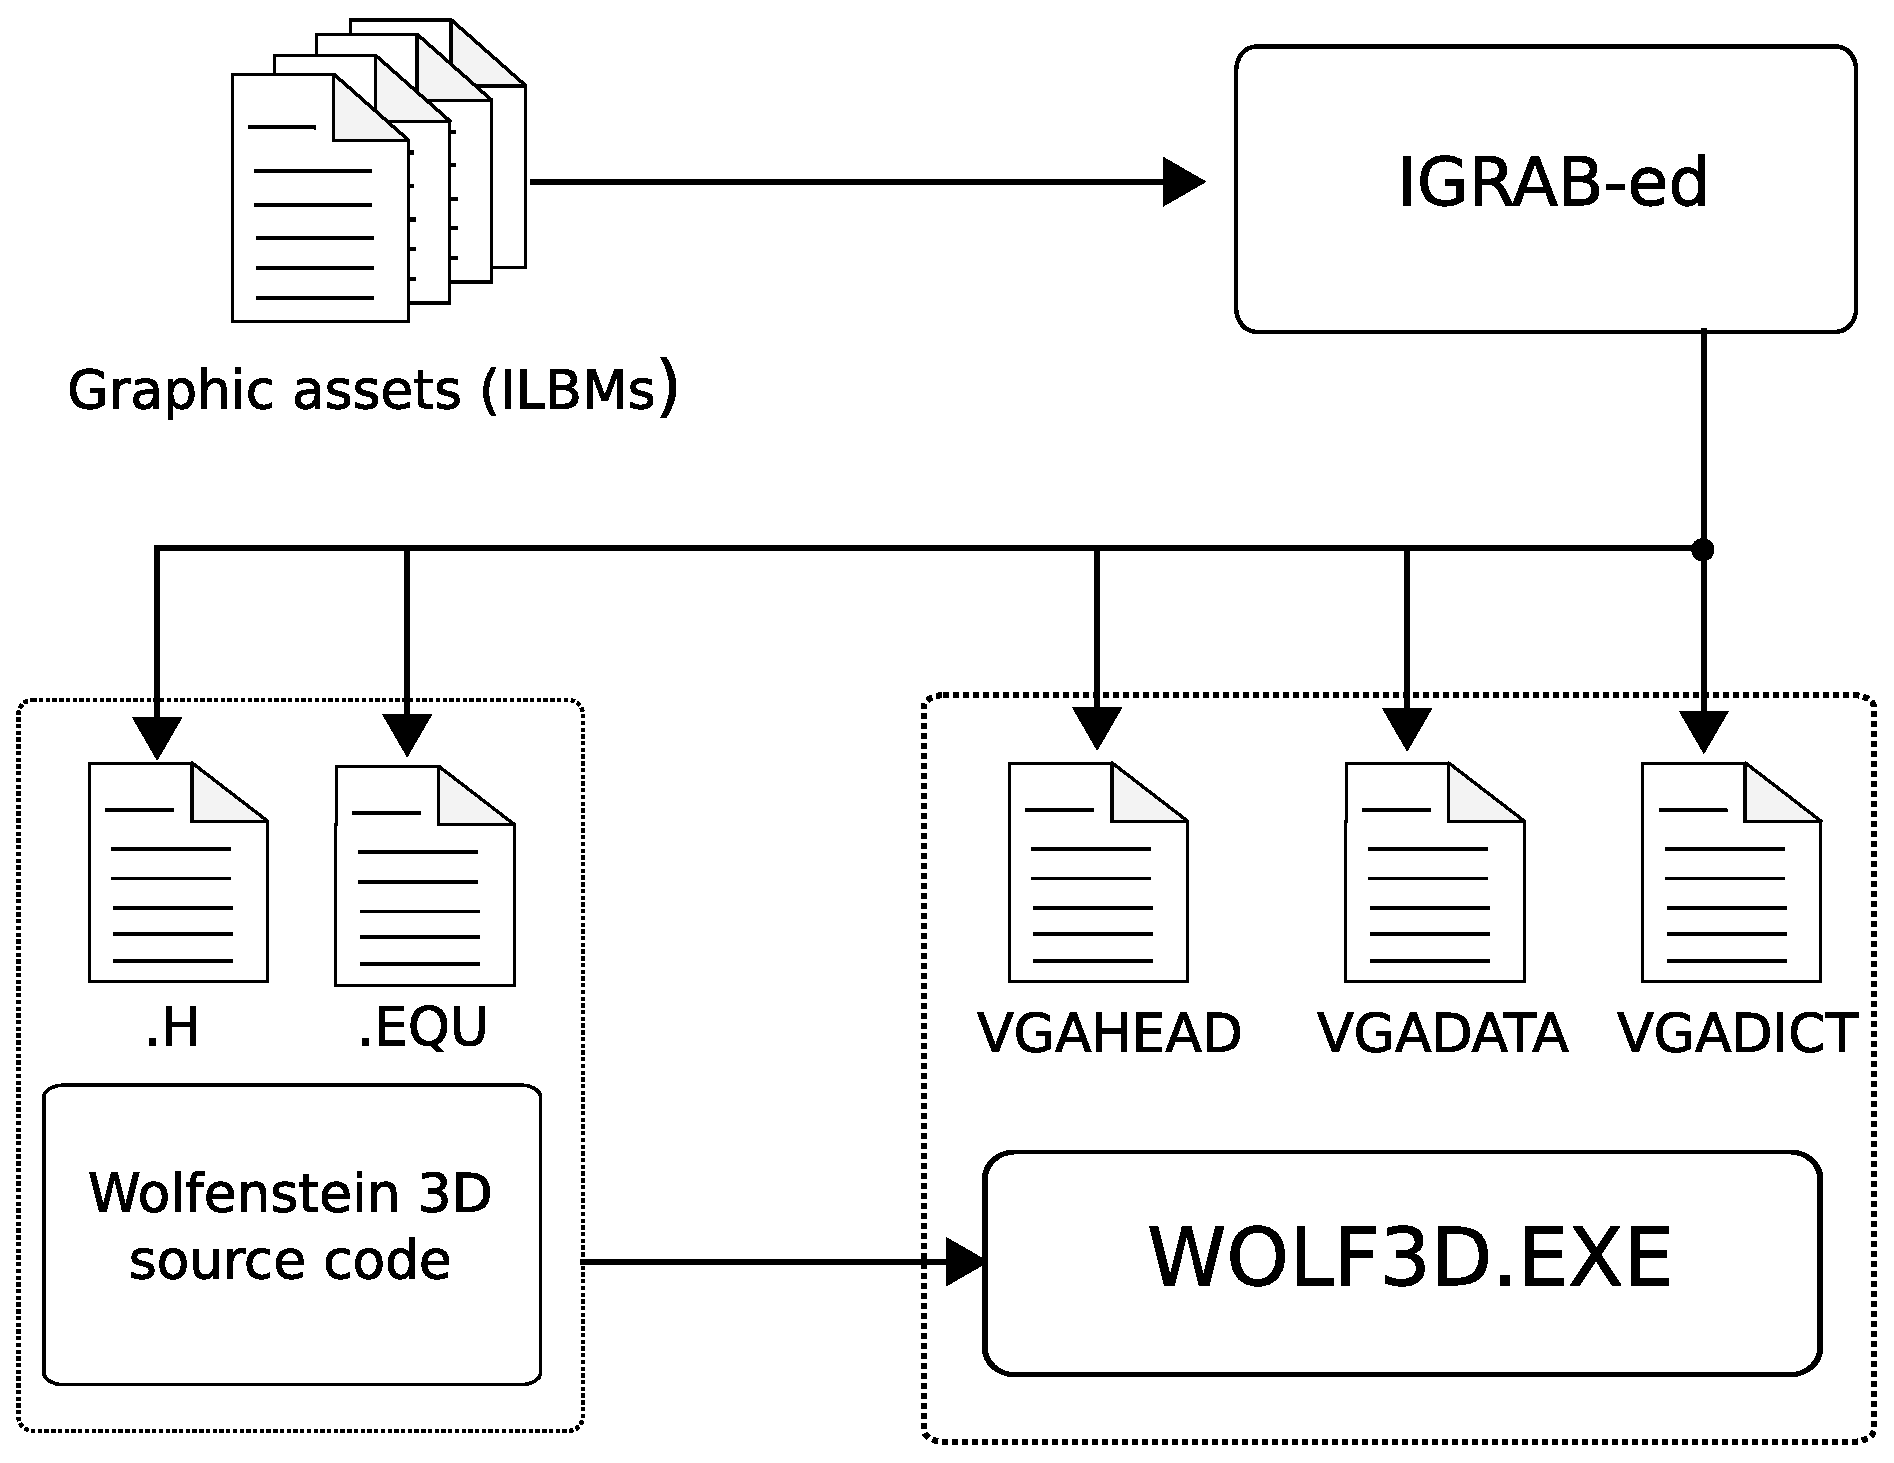
\includegraphics[width=.9\textwidth]{imgs/drawings/drawing_plain.eps}
 \caption{Asset creation pipeline for 2D Menu items}
 \label{asset-creation-pipeline}
\end{figure}
\par
\begin{minipage}{\textwidth}
 \lstinputlisting[language=C]{code/assets_header.c}\par
 \end{minipage}
 
 In the engine code, asset usage is hardcoded via an enum. This enum is an offset into the 
 \cw{HEAD} table which gives an offset in the \cw{DATA} archive. With this indirection layer, assets could be regenerated and reordered at will with no modification in the source code.\\
 \par
 \begin{minipage}{\textwidth}
 \lstinputlisting[language=C]{code/assets_usage.c}\par
 \end{minipage}


 
\pagebreak
\textbf{\underline{Trivia :}} This system led to issues when the source code was released. The \cw{.h} header files provided did not match the asset files from the shareware or early versions of Wolfenstein 3D. The headers released were from Spear of Destiny. You can see the kind of graphic mess this led to in the article "Let's compile like it's 1992" on \cw{fabiensanglard.net}.\\




\begin{minipage}{0.7\textwidth}
"The Official Hint Manual for Wolfenstein 3D" published in 1992 explains the creative process. It contains many drawings from Tom Hall and shows many behind the scene sketches made by Tom Hall and pixelarted by the graphic team.\\
\par
 \begin{fancyquotes}
When Id's Creative Director, Tom Hall gets an idea for a screen, he provides a sketch for Adrian Carmack. Below are some of Tom's early designs for the title screen. The third sketch was chosen.\\
\end{fancyquotes}
\end{minipage}
\begin{minipage}{0.3\textwidth}
\begin{flushright}
\scaledimage{0.9}{hint_manual_cover.png}
\end{flushright}
\end{minipage}

\noindent
   \begin{figure}[H]
\centering
 \fullimage{sprites/tom_hall_sketch_intro_screen_genesis.png}
 \par
 \scaledimage{.85}{sprites/woldf3d.png}
 \end{figure}
 \par
   

 





\label{hitler_drawing}
\begin{figure}[H]
\centering    
     \fullimage{sprites/tom_hall_sketch_adolf.png}
   \end{figure}



     \begin{figure}[H]
\centering
     \fullimage{sprites/tom_hall_sketch_dr_schabbs.png}
   \end{figure}
 
  \begin{figure}[H]
\centering
 \scaledimage{0.8}{sprites/tom_hall_sketch_gretel.png}\\
 \end{figure}



     \begin{figure}[H]
\centering
     \scaledimage{0.9}{sprites/tom_hall_sketch_giftmacher.png}
   \end{figure}

     \begin{figure}[H]
\centering
     \scaledimage{0.9}{sprites/tom_hall_sketch_fettgesic.png}
   \end{figure}


\par 
The hint manual also contains several photos of the team back in the day; it is worth a read for context\footnote{The manual was designed on a NeXT ColorStation. It was the only usage of Steve Jobs's machine for Wolfenstein 3D even though id purchased it in December 1991. NeXT series of workstations later became a key element of the production pipeline for Doom in 1992.}













\section{Maps}
Maps were created using an in-house editor called TED5, short for Tile EDitor. TED5 was not created specially for Wolf 3D, but was originally made for the Commander Keen series and improved over the years. It was a versatile tool since it allowed for creating maps of both side scroller games and top-down games like Rescue Rover and Wolf 3D. TED5 is not stand-alone; in order to start, it needs an asset archive and the  associated header (as described in the graphic asset workflow Figure \ref{asset-creation-pipeline} on page \pageref{asset-creation-pipeline}). This way, texture IDs are directly encoded in the map.\\

 \begin{figure}[H]
\centering
 \fullimage{TedSplashscreen.png}
 \end{figure}

  \begin{figure}[H]
\centering

 \fullimage{Fill_2.png}
 \end{figure}


 \begin{figure}[H]
\centering
 \fullimage{ted5_scrolling_map.png}
 %\caption{TED5 used for Commander Keen - side scroller.} 
 \end{figure}


\begin{figure}[H]
\centering
 \fullimage{TED.png}
 %\caption{TED5 used for top view level design in Rescue Rover.} 
 \end{figure}

 \par
 TED5 allows placement of tiles on layers called "planes". This layered approach proved powerful and versatile. In Commander Keen, layers are used for background, tiles which the hero can stand on, generating bonuses and so on. For Wolfenstein 3D, two layers are used: one for walls, and one to place bonuses and enemies on.\\
 \par

Reusing TED5 was a double win. Not only did it save tool development time, but ramp-up time was also reduced as all team members had been using it for years. TED5 was so good at doing the job that it allowed designers to make a level within minutes.\\
\par

 \begin{fancyquotes}
After talking with Romero and Tom, Scott learned that it was taking the group only about one day to make a level of the game. Ka-chung! Dollar signs! Instead of just three episodes, why not have six? Scott said, "If you can do thirty more levels, it would only take you fifteen days. And we could have it where people could buy the first trilogy for thirty-five dollars or get all six for fifty dollars, or if people buy the first episode and later want the second episodes it will be twenty dollars. So there's a reason to get them all!" After some consideration, id agreed.\\
\\
 \textbf{- Masters of Doom}
 \end{fancyquotes}\\

\par
While everybody worked a little bit on the map, it was mostly the creation of John Romero and Tom Hall.\\
\par
 \textbf{\underline{Trivia :}} The source code of TED5 was released several years later. Among the source code made of \cw{.C} and \cw{.H} was a mysterious \codeword{\_TOM.PIC}\footnote{Intentionally not reproduced here.}. It turned out to be an adult caricature of Tom Hall made by Adrian Carmack. The explanation was provided later by John Romero in 2002:\\
\par
 \begin{fancyquotes}
   "Hahahaha! Wow, I forgot all about that picture. I can't believe it's 
in the TED5 source files! It's basically a pic that Adrian drew of Tom 
[...] saying "Sorry!".\\
\par 
It's because Tom and Adrian used to share a worktable together and Tom 
would always bump the table while Adrian was drawing graphics with the 
mouse and Tom would say, "Sorry!" That picture never appears in TED5 
anywhere.\\
   \\
\textbf{John Romero - Programmer}
 \end{fancyquotes}











\section{Audio}

\subsection{Sounds}
As mentioned in Chapter \ref{hardware-audio}, audio hardware was highly fragmented. id decided to support four sound cards and the default PC speaker, which meant generating assets multiple times for each and packing them together with an in-house tool called MUSE into an AUDIOT archive (an id software proprietary format):\\
\begin{figure}[H]
\centering

   \fullimage{muse.png}
  \caption{MUSE splash screen.}
 \end{figure}
 \par
 Three sets of each audio effect shipped with the game:
\begin{enumerate}
\item For PC Speaker
\item For AdLib
\item For SoundBlaster, SoundBlaster Pro and Disney Sound Source
\end{enumerate}

\par
All voices were recorded by John Romero and Tom Hall faking German accents\footnote{Masters of Doom by David Kushner.} the best they could\footnote{You can actually recognize their voices if you listen carefully: Tom Hall's "guten tag" is memorable.}.






\subsection{Music}
All music composition was done by Robert Prince.\\
\par
 \begin{fancyquotes}
In the early days of the OPL soundcards, the "gold standard" sequencing software was Sequencer Plus Gold ("SPG") by Voyetra. The reason for this was it had an OPL instrument/instrument bank editor.\\
\par
To rough out compositions, I used Cakewalk ("CW"). I had been using it for several years already and had it all set up to use the analog boxes for sound output. Having "real" sounds from those boxes helped me visualize (audiolize?) what I wanted musically. I would save the CW files in *.mid format and load them into SPG to create the OPL instrument for each track. I built different instrument banks for the different genres of music.\\
\par

\textbf{Bobby Prince - Composer}
 \end{fancyquotes}\\
 \par
\begin{figure}[H]
\centering

 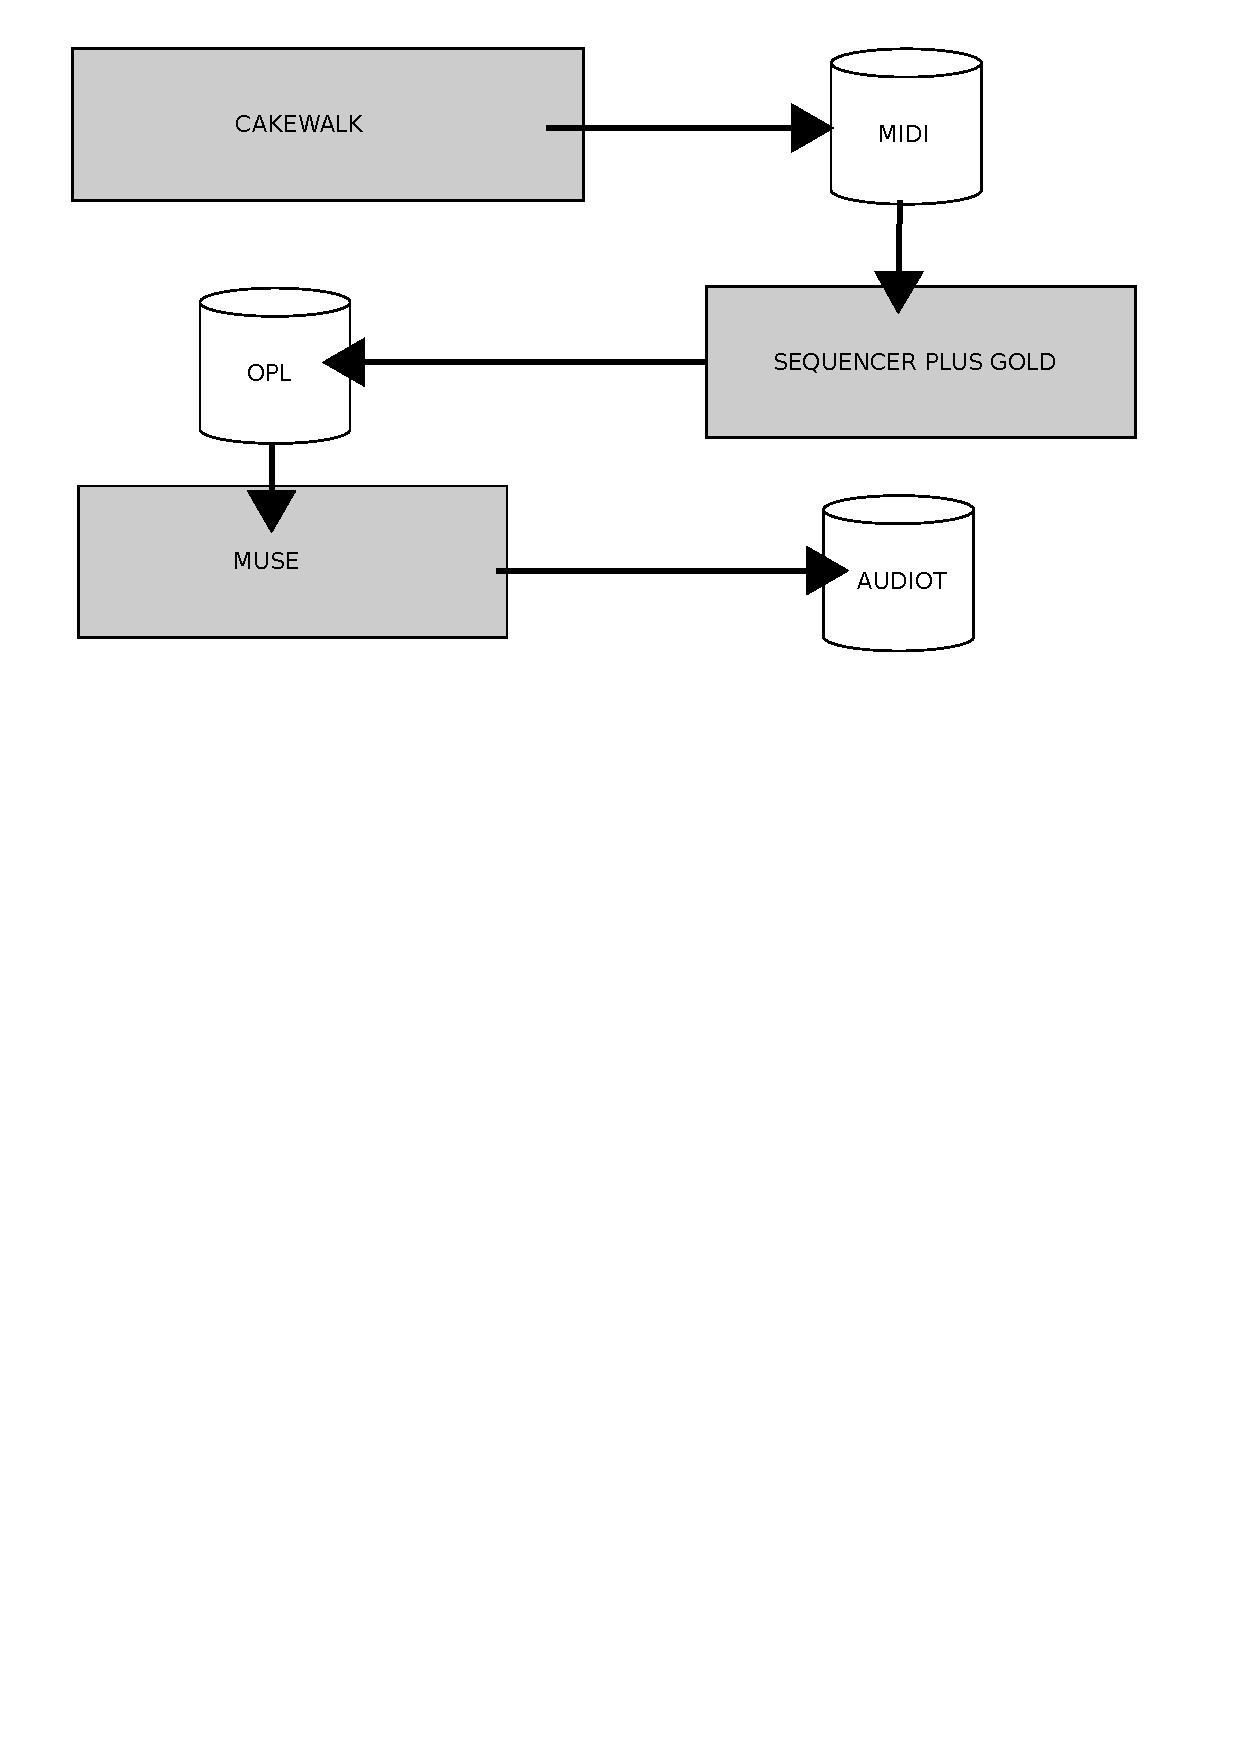
\includegraphics[width=0.9\textwidth]{imgs/drawings/music_pipelione.pdf}
 \caption{Music pipeline as described by Bobby Prince.}
\end{figure}
\par


\begin{figure}[H]
\centering
      \scaledimage{1}{music_editor.png}
\caption{Sequencer Plus Gold ("SPG") by Voyetra.}
\end{figure}


What goes in the \cw{AUDIOT} archive is a music format called IMF\footnote{Id software Music File.}. As it supports only the YM3812, it is tailored for the chip with zero abstraction layer. It consists of a stream of machine language commands with associated delays\footnote{IMF format is explained in detail on page \pageref{IMF_explanation}}.\\
\par
 The stream pilots the nine channels in the OPL2. A channel is able to simulate an instrument and play notes thanks to two oscillators, one playing the role of a modulator and the other the role of a carrier. There are many other ways to control a channel such as envelope, frequency or octave.\\
\par The way a channel is programmed is described in detail in Section \ref{IMF_explanation}, "\nameref{IMF_explanation}" on page \pageref{IMF_explanation}.\\
\par
LGSDGLASFLDSA
\pagebreak


\begin{figure}[H]
\centering
 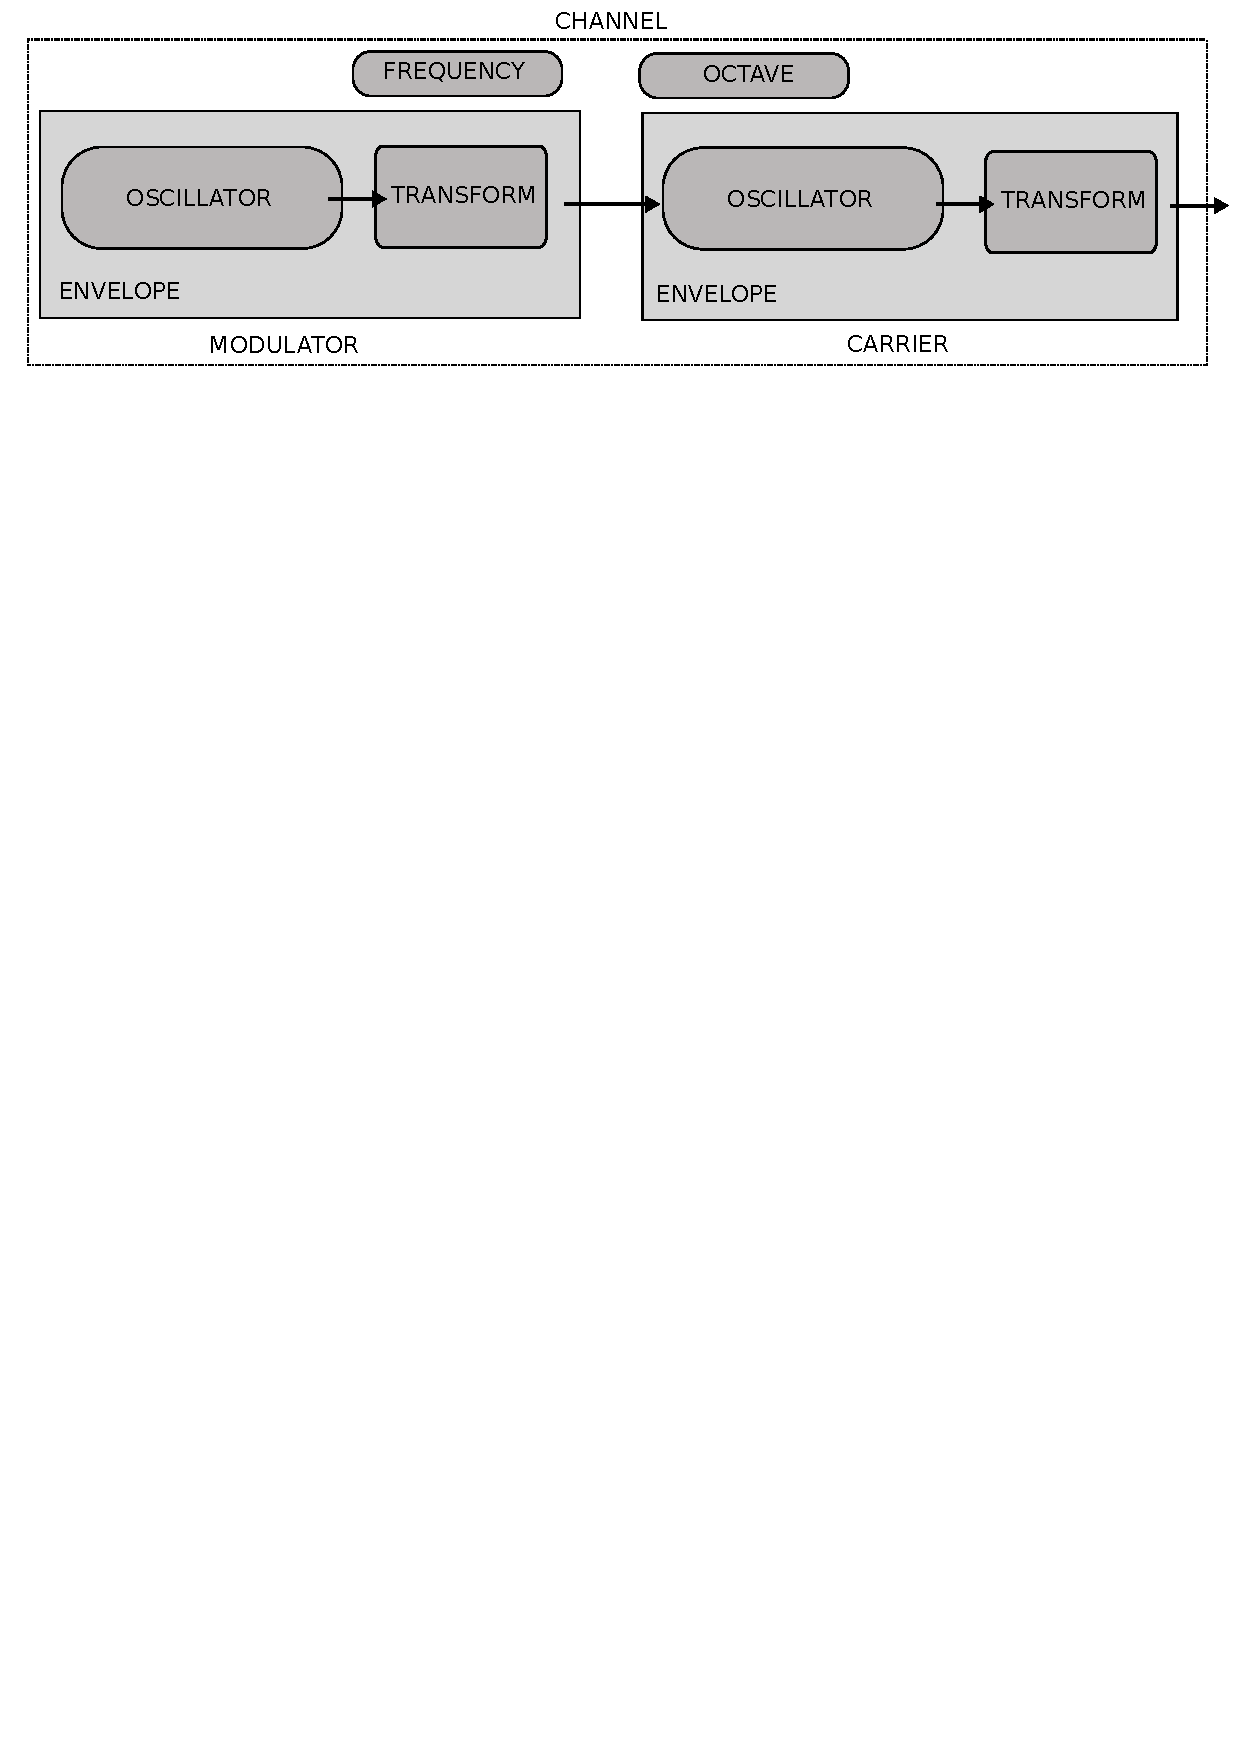
\includegraphics[width=\textwidth]{imgs/drawings/channel.pdf}
 \caption{Architecture of a YM3812 channel.}
\end{figure}
\par
\bu{Trivia :}  The YM3812's unmistakable sonority is due to its peculiar set of waveform transformers (they are right after the output of each oscillator in the drawing). Four waveforms are available on the OPL2: Sin \circled{1}, Abs-sin\circled{2}, Pulse-sin \circled{3}, and Half-sin \circled{4}.
\par
\begin{figure}[H]
\centering
 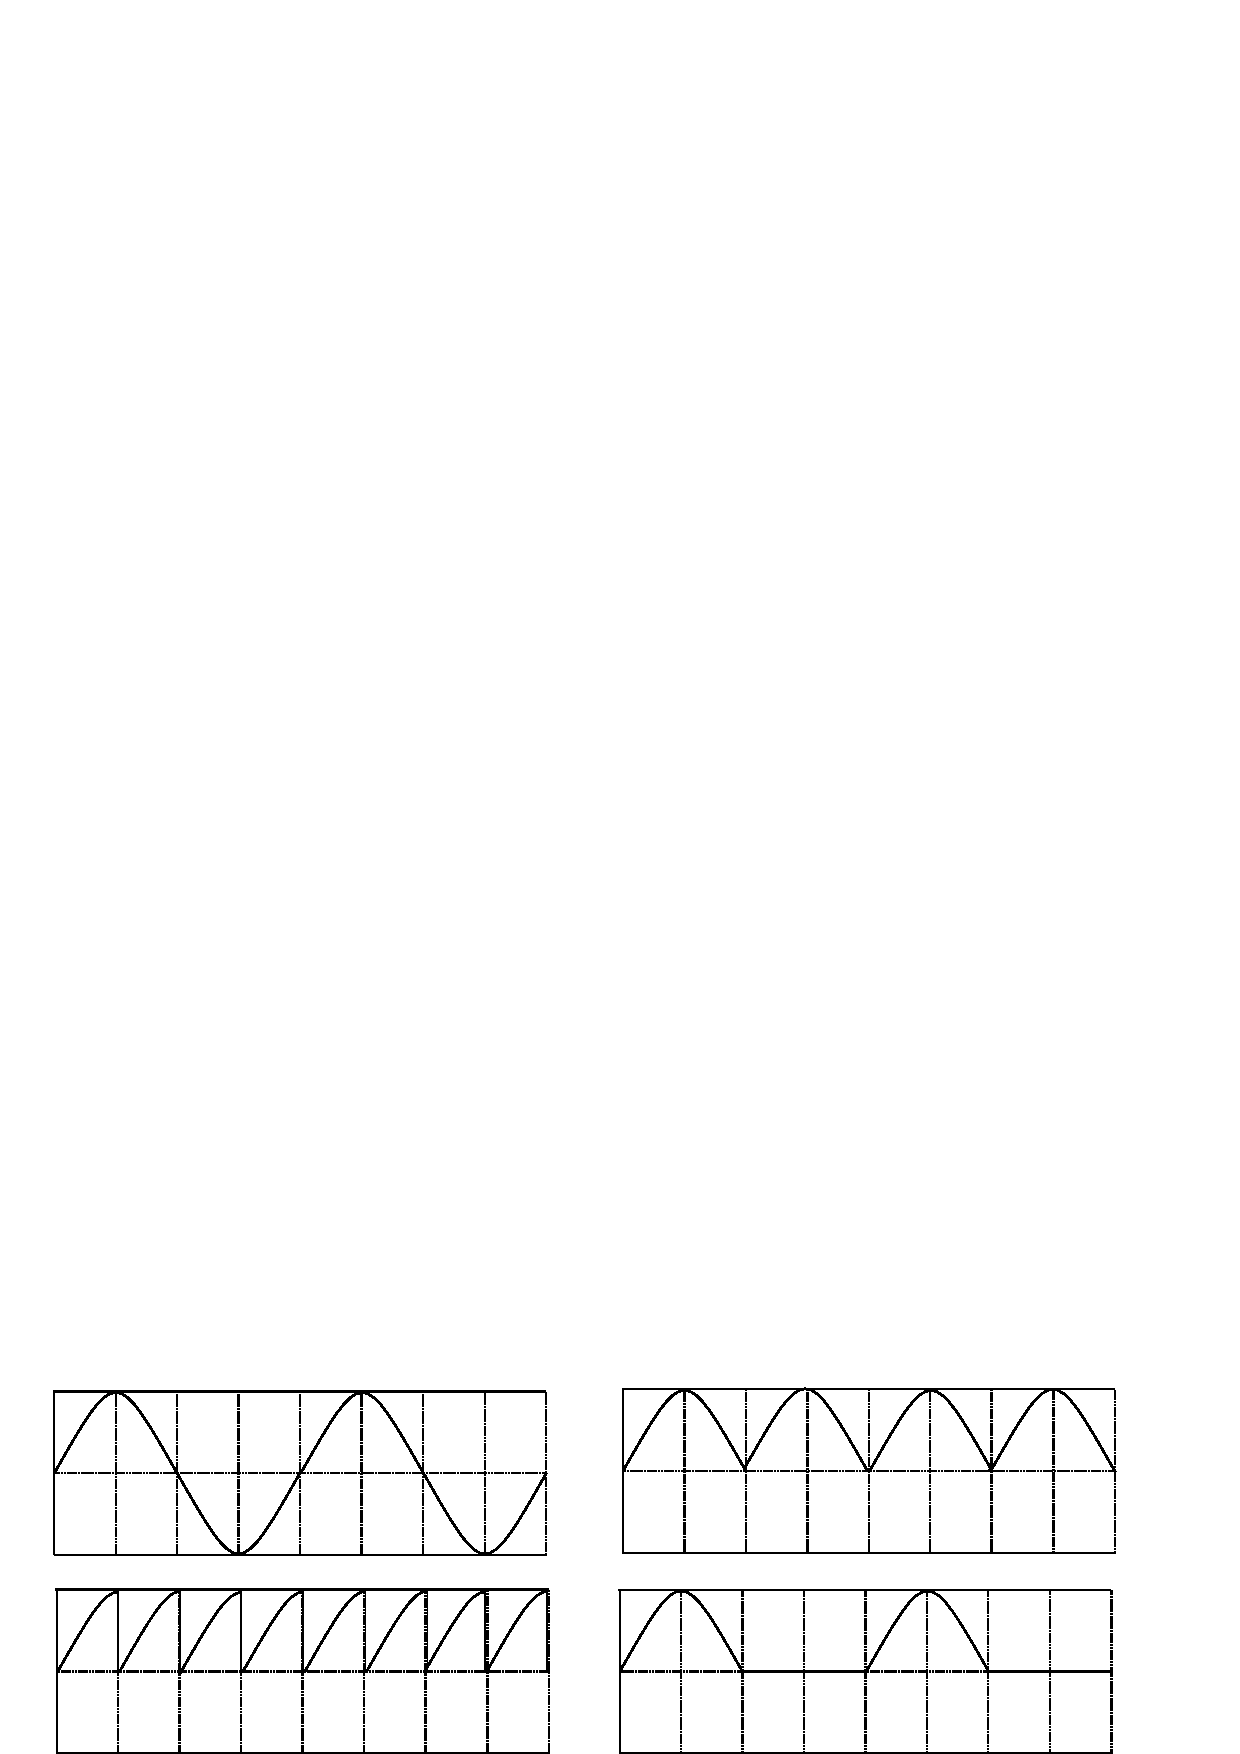
\includegraphics[width=\textwidth]{imgs/drawings/wave_transform.pdf}
 \caption{The four waveform transforms available.}
\end{figure}


\bu{Trivia :} In Episode 3 the music playing features a hidden Morse code message. "To Big Bad Wolf. De Little Red Riding Hood. Eliminate Hitler. Imperative. Complete mission within 24 hours. Out." The end boss of this episode is indeed Hitler in a Mech suit (see hint manual drawing on page \pageref{hitler_drawing}).




























\section{Distribution}
At 4am on May 5th, 1992 the first episode of the game was uploaded to Massachusetts via Software Creations BBS\footnote{Bulletin Board Systems where server allows users to connect via a console and upload/download programs.} server. Wolfenstein 3D was distributed as shareware; the game engine and first episode were given for free and encouraged to be copied and distributed to a maximum number of people. To receive the five other episodes, each player had to pay \$50 to id Software.\\
\par
\begin{figure}[H]
\centering
 \fullimage{shareware.png}
 \caption{Exiting the game describes how to get the full version.}
 \end{figure}

\end{document}
\par
In order to maximize income, it was therefore paramount to make the game easy to copy and redistribute. In 1991, Internet was still in its infancy and the best medium was the 3\nicefrac{1}{2}-inch floppy disk. Particular attention was given to the total size of the game so it would fit on one disk. All assets combined accounted for 1,204KiB but everything was compressed to 645KiB (a 3\nicefrac{1}{2}-inch floppy can store 720KiB). The full six episodes fit on two disks. Spear of Destiny would fit on three disks.
The game shipped as follows:\\

  \par
 The files can be divided in five parts:
 \begin{itemize}
 \item WOLF3D.EXE: Game engine.
 \item VSWAP.WL1: Contains all the assets (sprites, textures, digitized sounds) needed during 3D action phases.
 \item Music and sound effect files used during both 3D and 2D phases:
     \begin{itemize}
     \item AUDIOHED.WL1 : Index to payload in \cw{AUDIOT} file.
     \item AUDIOT.WL1: Uncompressed audio data. 
     \end{itemize}
\item Maps:
     \begin{itemize}
     \item MAPHEAD.WL1 : Index into \cw{GAMEMAPS} file.
      \item GAMEMAPS.WL1 : Compressed Map payloads.
      \end{itemize}
\item Pictures used during 2D menu phase:
    \begin{itemize} 
    \item VGAHEAD.WL1 : Index into \cw{VGAGRAPH} file.
    \item VGADICT.WL1 : Huffman-tree to decompress each picture.
    \item VGAGRAPH.WL1 : Compressed pics lumped together.
     \end{itemize}
\end{itemize}

\par
 \begin{figure}[H]
\centering
 \fullimage{result.png}
 \caption{All files distributed as shareware as they appear in DOS command prompt.}
  \end{figure}
 \par

\pagebreak
\textbf{\underline{Trivia :}} The file extensions did have meaning: 
\begin{itemize}
\item WL1: Shareware.
\item WL3: Early three-episode full version (never released).
\item WL6: Six-episode full version.
\item WJ1: Japanese shareware.
\item WJ6: Japanese full version.
\item SOD: Spear of Destiny.
\end{itemize}
 
\textbf{\underline{Trivia :}} The engine is very tiny and only uses 94KiB in total. But with 64KiB dedicated to the \cw{Signon} screen (and 768B for the palette), the engine is in fact only 29KiB.\\
\par
\begin{figure}[H]
\centering
\scaledimage{0.7}{disk.png}\\
\end{figure}
\par
On the previous page is an image of a 3\nicefrac{1}{2}-inch floppy widely used to share and redistribute the game. The upper left hole allows the disk reader to recognize if the disk is a low capacity (full = 720 KiB) or a high capacity (hole = 1.44 MiB version). The upper right hole features a sliding tab which when closed forbids writing to the disk, making it read-only. Once inserted in the floppy disk reader, the large metallic tab slides to the right to expose the magnetic disk.\\
\par
\textbf{\underline{Trivia :}} Some people (including the author) saved money by drilling holes in their 720 KiB certified floppy disks to have them recognized as 1.44 MiB. It worked!
